
\section{Kohlenhydrate} \label{sec:kohlenhydrate}

Kohlenhydrate enden auf -ose. \\
Jedes C-Atom darf nur eine Hydroxy-Gruppe haben. \\
Folgendes gilt für Kohlenhydrate:
\begin{itemize}
    \item Zahl der C-Atome:
        \begin{itemize}
            \item 3: Triose
            \item 4: Tetrose
            \item 5: Pentose
            \item 6: Hexose
        \end{itemize}
    \item Zahl der Einheiten:
        \begin{itemize}
            \item 1 Zuckereinheit: Monosaccharid
            \item 2 Zuckereinheiten: Disaccharid
            \item 3-20 Zuckereinheiten: Oligosaccharid
            \item 20 \textless\ Zuckereinheiten: Polysaccharid
        \end{itemize}
    \item Nach ihrer funktionellen Gruppe:
        \begin{itemize}
            \item Aldehydgruppe:
                \begin{itemize}
                    \item Aldosen
                    \item Glucosen
                    \item Polyhydroxyaldehyde
                \end{itemize}
            \item Ketogruppe:
                \begin{itemize}
                    \item Ketosen
                    \item Fructosen
                    \item Polyhydroxyketone
                \end{itemize}
            \item =\textgreater\ sie sind das Produkt der partiellen Oxidation mehrwertiger Alkohole
        \end{itemize}
\end{itemize}

\subsubsection{Zu merkdende Kohlenhydrate:}
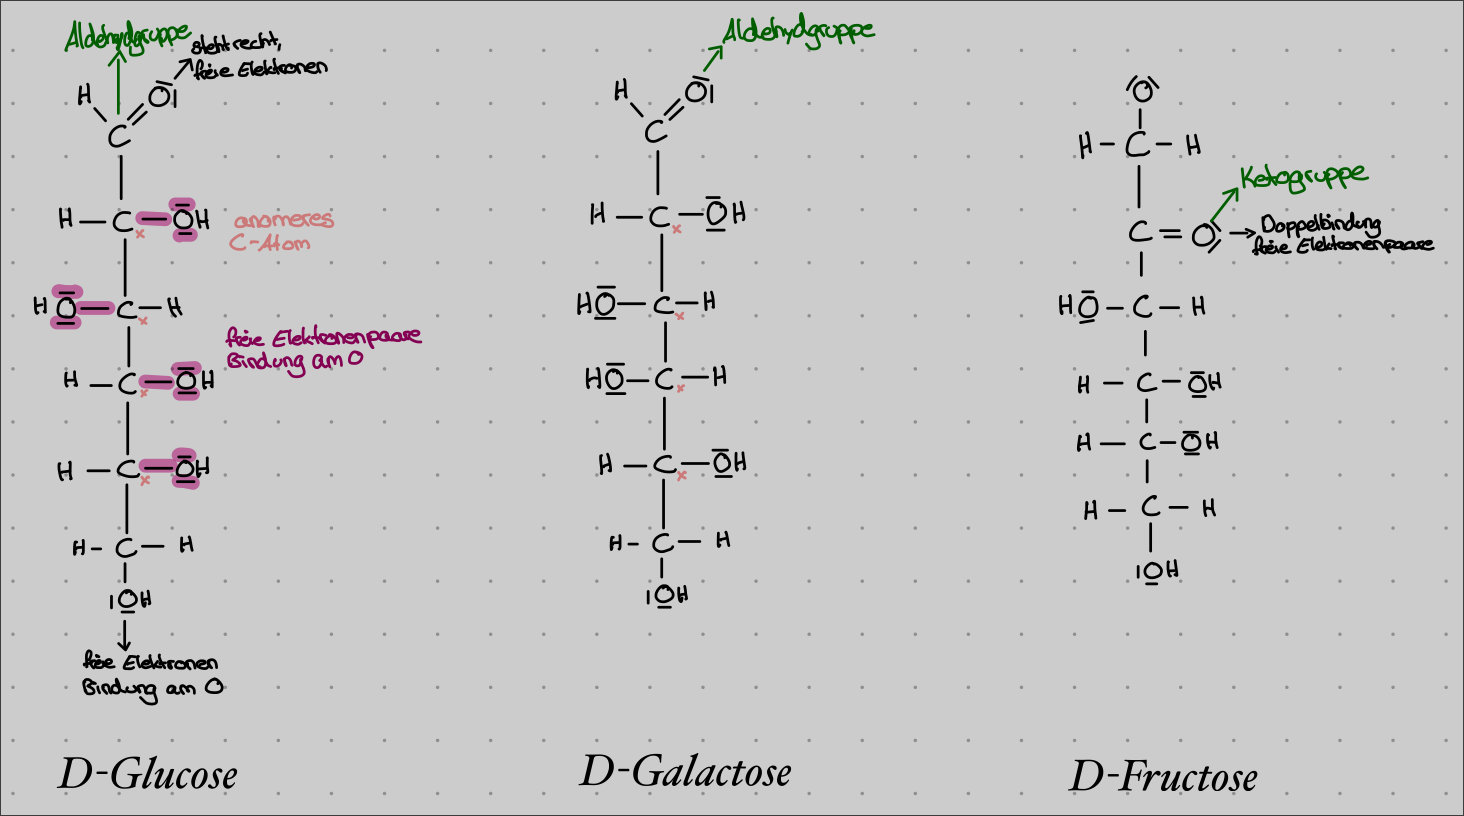
\includegraphics[scale=0.31]{media/naturstoffe/stoffe.png}
